%%%%%%%%%%%%%%%%%%%% Chapter 3
\chapter{Lasso Gripper: Design, Analysis, and Experiments}

\begin{chaptersummary}
This chapter presents Lasso Gripper as the primary mechanism study and principal novel end-effector concept of this thesis. It is used to investigate tendon-driven design principles and evaluate the feasibility of a controllable tensile loop as a practical robotic end-effector. The concept was inspired by the observation of a toy that launches a flexible string into the air, where manual motion can alter the loop shape and occasionally produce a relatively stable free-space loop. This observation motivated the conversion of a projected loop into an actively retractable capture mechanism. The chapter covers the device concept, mechanical architecture, actuation and sensing design, grasp planning strategy, and a series of demonstration experiments, while also analyzing the fundamental dynamics governing the formation and stability of the self-supporting string loop that enables the gripper to operate.

An analytical model based on a Frenet-Serret formulation is developed to describe the loop behavior by balancing tension, gravity, and aerodynamic drag, allowing identification of loop-formation regimes and critical transition points. Key assumptions and simplifications, including negligible string radius and linear drag approximation, are explicitly stated, and representative experimental observations are used to validate the predicted trends. Together, the modeling and experimental analyses reveal mechanism-level advantages, operational constraints, and potential failure modes that inform the broader thesis on tendon-driven robotic systems.

The experimental program is demonstration-focused and qualitative by design, illustrating the gripper's operating behaviors, tolerance to object uncertainty, and comparative advantages over a conventional antipodal gripper. Comprehensive quantitative evaluation, including large-sample success-rate analysis, repeatability assessment, and detailed parametric sensitivity studies is beyond the scope of this chapter and is recommended for future work.
\end{chaptersummary}
% ------------------------- 2.1 Overall Structure -------------------------
\section{Concept and Design Requirements}

\subsection{Design Inspiration and Concept Formation}

The initial inspiration for Lasso Gripper came from a toy rather than from a conventional robotic gripper. The toy could launch a length of string into the air. By moving the handheld part, the user could change the shape of the airborne string loop, and under certain motions the loop could appear relatively stable for a short period. The toy itself was not a grasping device, and it did not actively tighten around objects. However, the observed phenomenon suggested an important mechanism idea: a flexible string can form a controllable spatial loop when its motion, gravity, aerodynamic drag, and internal tension are appropriately balanced.

This observation was abstracted into a robotic design question. If an airborne loop can be produced in a repeatable way, and if the loop can subsequently be retracted under controlled tension, then the loop may act as a projected capture region rather than a conventional pair of rigid fingers. The robotic concept therefore adds two functions that the toy did not provide: controlled launch and active retraction. Launch creates the open loop in free space, while retraction converts loose enclosure into holding force.

The key mechanism transition is from \emph{free-space loop formation} to \emph{loop-based grasping}. In the toy, the loop is mainly a dynamic visual and physical phenomenon. In Lasso Gripper, the same type of loop is treated as a temporary end-effector geometry. The loop first increases the region in which an object can be captured, and the tightening stage then transforms this region-level interaction into a stable grasp or hold. This design path is important because it separates the source of inspiration from the final robotic function: the contribution is not the toy itself, but the conversion of a free string loop into a controllable capture-and-retraction mechanism.

\subsection{Design Requirements for Robotic Loop Capture}

Translating the toy-inspired phenomenon into a robotic gripper required several design requirements. First, the device had to create a capture region larger than the physical body of the end-effector. This requirement distinguishes Lasso Gripper from parallel-jaw grippers, whose effective capture area is limited by jaw opening and fingertip placement. Second, the loop had to tolerate object-position uncertainty. The intended advantage of the mechanism is not high fingertip precision, but the ability to sweep a loop across a broader target region and then tighten around a useful feature.

Third, the string had to remain light enough for rapid launch and free-space loop formation. A heavy string would sag quickly and reduce the projected capture envelope. Fourth, the string surface had to provide enough interaction with both the driving wheels and the surrounding air. Sufficient wheel friction is needed for repeatable propulsion, while aerodynamic drag contributes to the self-supporting loop behavior analyzed later in this chapter. Fifth, the mechanism had to include active retraction, because a loop that can only be launched cannot reliably generate holding force. Finally, the distal structure had to remain mechanically simple so that the system could be mounted on a robot arm without adding heavy or bulky fingers at the interaction point.

\begin{description}[style=standard, leftmargin=1.5em, labelindent=0pt, itemsep=0.6em]
    \item[\textbf{Large capture envelope:}] The loop should create an interaction region larger than the rigid body of the gripper.

    \item[\textbf{Tolerance to pose uncertainty:}] The mechanism should not require precise antipodal contact placement before capture.

    \item[\textbf{Low string mass:}] The string should be light enough to form a free-space loop during launch rather than immediately collapsing under gravity.

    \item[\textbf{Sufficient friction and aerodynamic interaction:}] The string should be rough enough for reliable friction-wheel propulsion and should interact with air strongly enough to support loop formation.

    \item[\textbf{Active retraction:}] The mechanism must tighten the loop after placement so that enclosure can become a stable grasp.

    \item[\textbf{Low distal complexity:}] The gripper should keep the capture structure flexible and lightweight, with actuation and sensing located proximally where possible.
\end{description}

\subsection{String Material Screening}

Early qualitative trials were conducted to evaluate both string behavior and wheel-string interaction. Candidate string materials included cotton string, fishing line, nylon line, and silicone cord. These trials were used as design screening rather than formal experiments. They were not recorded with video or image documentation and are therefore not treated as quantitative validation evidence. Their purpose was to identify a string and launch-interface combination that could be driven reliably, form a visible and controllable loop, and retract without excessive tangling or slipping.

The original toy used ABS launching wheels. Their surface friction was insufficient under some string conditions, and slipping could occur during launch. Silicone cord was therefore considered because its compliant and high-friction surface could improve engagement with the wheels. However, the silicone cord was too heavy for the desired free-space loop behavior and was less suitable for rapid launch. This observation separated the design problem into two parts: the string should remain light and flexible, while the launching wheel should provide sufficient surface grip. Fishing line was relatively smooth and tended to retain curvature, making it less suitable for stable loop formation. Nylon line was also comparatively smooth, which reduced the reliability of wheel-string interaction. Cotton string provided the best practical balance in the prototype trials. It was light, flexible, and sufficiently rough to interact with both the launch mechanism and the surrounding air. The later prototype therefore used cotton string together with patterned TPU launching wheels, as described in the mechanical design, to improve propulsion reliability without increasing string mass.

This material choice is closely related to the mechanism principle. The string is not merely a passive connector; it is the temporary grasping structure. Its mass, surface texture, flexibility, and bending behavior directly influence launch consistency, loop stability, retraction behavior, and object contact. Therefore, string material selection is part of the mechanism design rather than a secondary implementation detail.

\section{Prototype Architecture and Working Mechanism}

After defining the design requirements, this section describes how the prototype realizes the loop-based grasping concept in hardware. The discussion first presents the system architecture, then explains the capture mechanism, the string shooting and retraction unit, and the controller and sensing hardware that execute the grasping sequence.

\subsection{Overall Prototype Architecture}

\begin{figure}[htbp]
\centering
\begin{tabular}{cc}
\begin{minipage}[t]{0.9\textwidth}
\centering
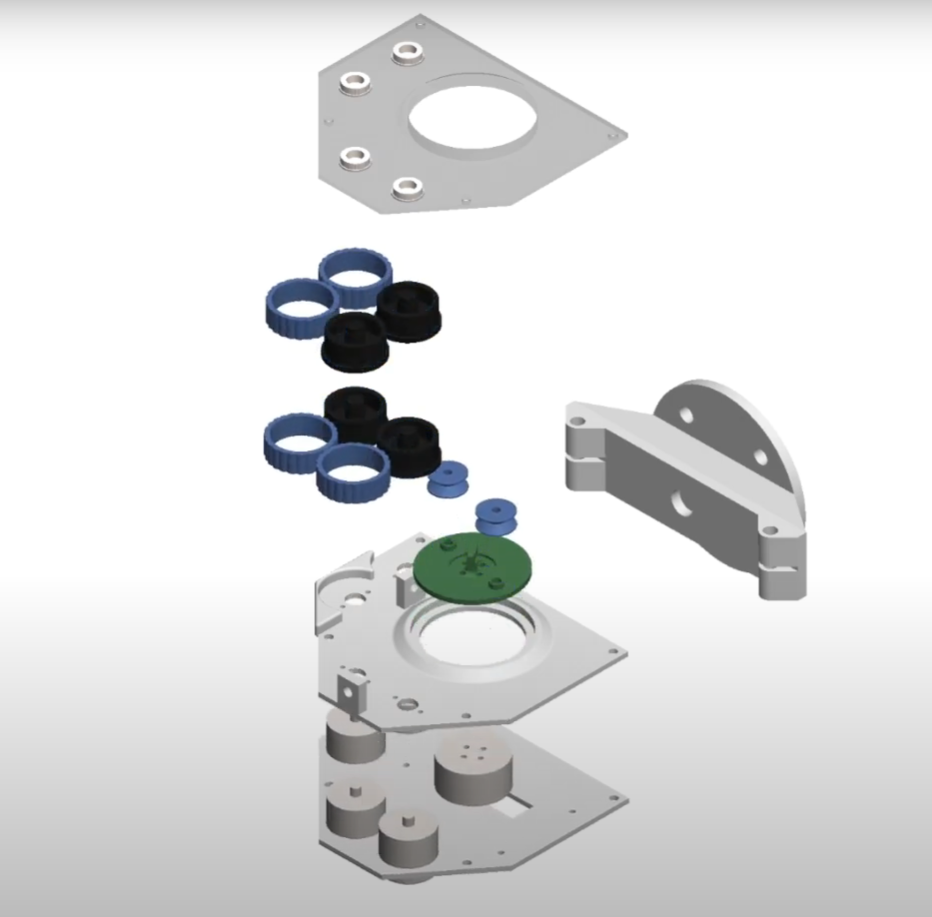
\includegraphics[width=\linewidth]{Figures/overall_img.png}
\caption{The SolidWorks designed hardware of the proposed gripper}
\end{minipage}
\end{tabular}
\end{figure}

Lasso Gripper integrates four core subsystems: the launch-and-retract end-effector, a proximal control unit, sensing for tension and loop position, and a host robot for gross positioning. The end-effector implements the friction-wheel propulsion and spool retraction mechanisms; the control unit coordinates motor commands and processes sensor feedback; sensing includes a spool-mounted force sensor and motor/position encoders used for tension regulation; the host robot provides coarse positioning and aiming for capture. This modular decomposition clarifies subsystem responsibilities and guides the experimental evaluation reported below.

\begin{figure}[htbp]
\centering
\begin{tabular}{cc}
\begin{minipage}[t]{0.9\textwidth}
\centering
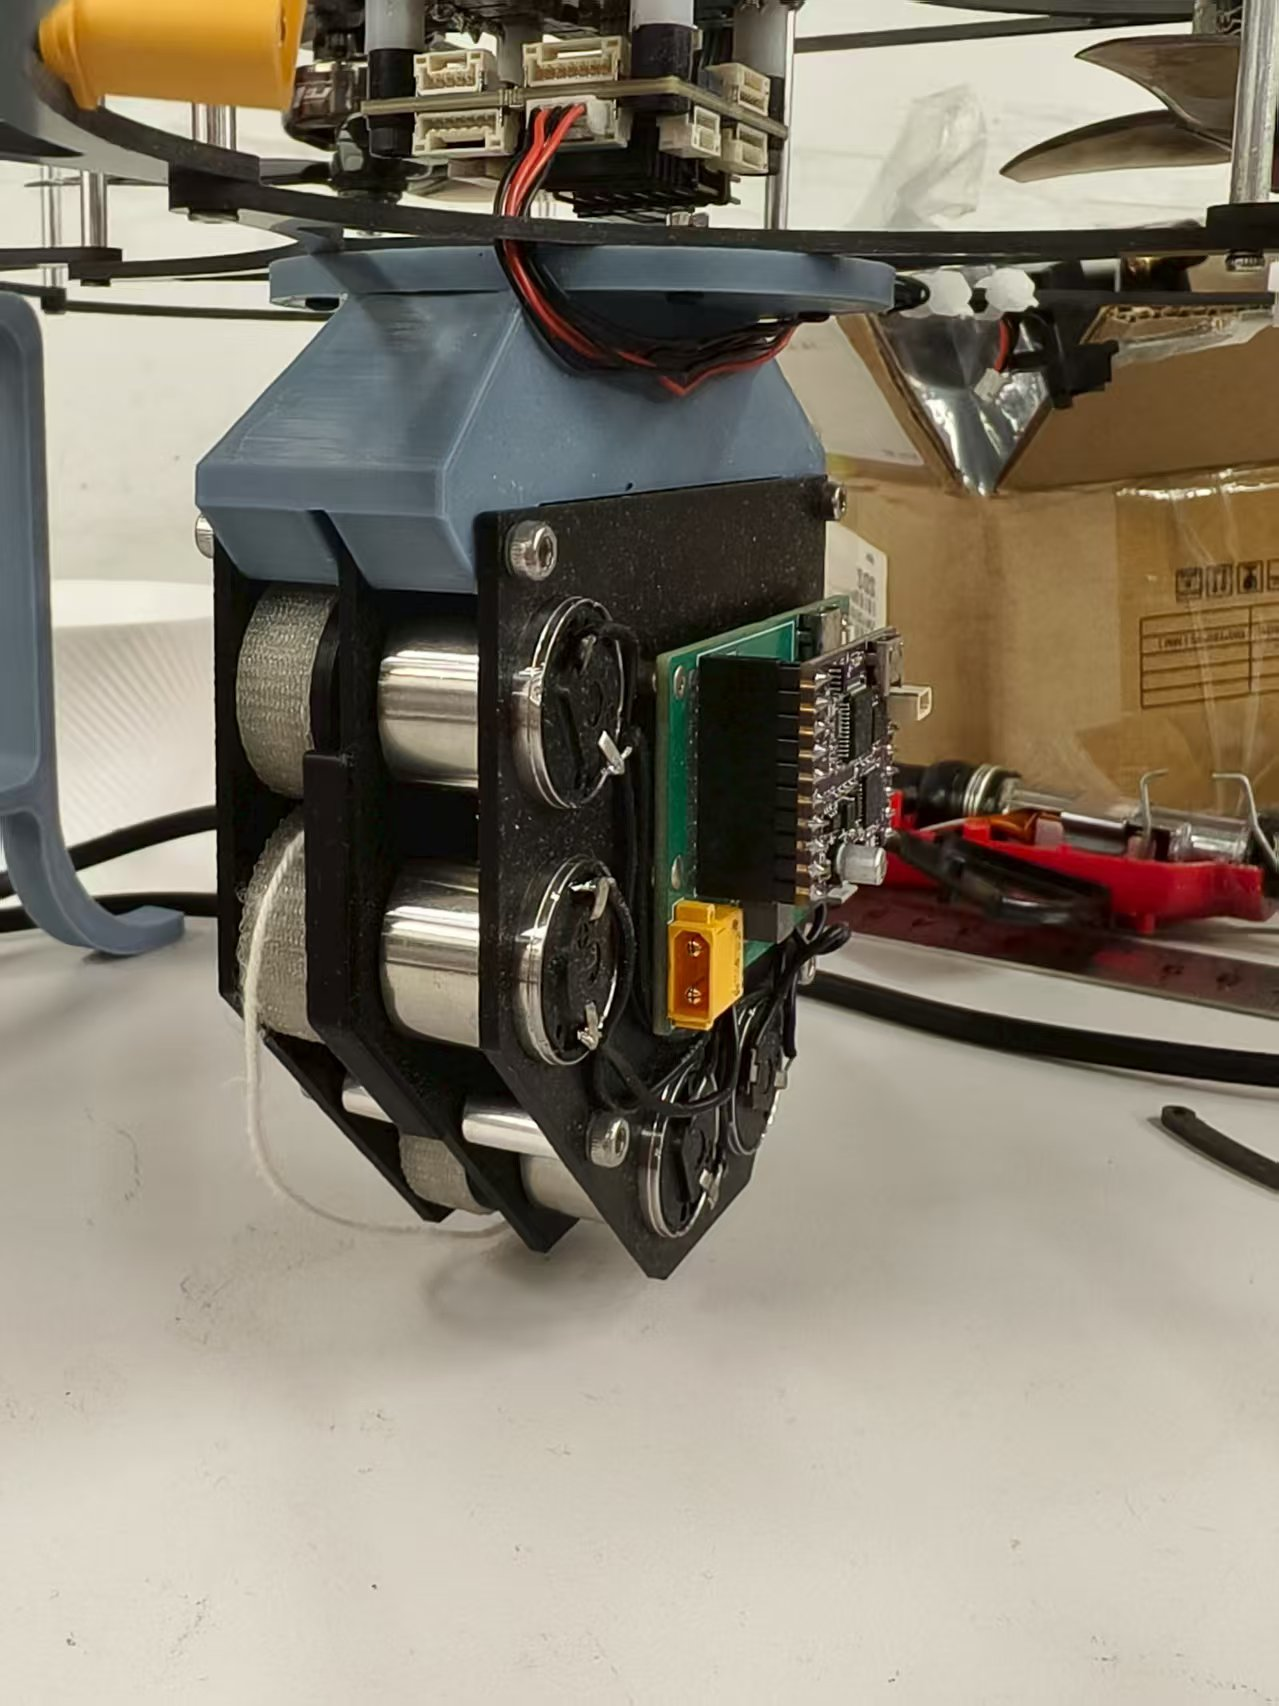
\includegraphics[width=\linewidth]{Figures/system_overview.jpg}
\caption{The proposed gripper connected with an ESP32 controller, motor electronic speed controller.}
\end{minipage}
\end{tabular}
\end{figure}

\subsection{Mechanism of Loop-Based Capture}

The grasping principle of Lasso Gripper differs from classical antipodal grasping. A parallel-jaw gripper typically requires two suitable contact regions and relatively accurate fingertip placement. Lasso Gripper first creates a projected loop, which acts as a large capture envelope. If the loop passes around a neck, protrusion, frame, or enclosed region of the target, subsequent retraction can convert the loose loop into a tightened contact path.

This process can be understood in three phases. In the deployment phase, the launched string forms an open loop in free space. In the enclosure phase, the robot motion or target motion causes the object to enter the loop region. In the tightening phase, the spool retracts the string and increases tension, causing the loop to close around the target. The result is not a two-point contact grasp but a distributed contact interaction along part of the string path.

This distributed contact is the main source of the gripper's advantage for deformable, oversized, and irregular objects. For a deformable object, the string can spread contact over a longer path and reduce local pressure compared with rigid fingertips. For a frame-like object, the loop can pass through or around an opening and then tighten on the frame. For an oversized object, the loop can partially enclose or hook a useful region even when the object is larger than the rigid body of the gripper. For a moving object, the open loop increases the temporal and spatial window for capture, provided that launch and retraction timing are selected appropriately.

The mechanism also has inherent limitations. A loop that misses the target region cannot generate grasping force. A loop that tightens above an unstable center-of-mass relationship can slip during lifting. Excessive retraction can damage soft targets, while insufficient retraction can leave the object unsecured. These limitations motivate the control assumptions, parameter selection, and failure analysis presented later in this chapter.



% ------------------------- 2.2 String Shooting and Retraction Mechanism -------------------------
\subsection{String Shooting and Retraction Mechanism}

The string shooting and retraction mechanism is a defining feature of Lasso Gripper, enabling it to perform complex gripping tasks with high efficiency. The mechanism comprises multiple components working in unison to achieve precise control over the string's movement.

The propulsion of the string is achieved through two pairs of friction wheels. These wheels are designed with high-friction surfaces to grip the string effectively. The wheels are driven by coreless motors with high speed so that the required rotational speeds for rapid string extrusion can be achieved\cite{murata2024elastic}.

During the string shooting phase, both pairs of friction wheels rotate in the same direction, propelling the string forward through a guided track. This track is designed to help the string form a loop within the desired dimensions and shape. In the prototype reported here, the launch duration and wheel speeds were specified by the experiment script rather than adjusted by online visual recognition.

\begin{figure}[htbp]
\centering
\begin{tabular}{cc}
\begin{minipage}[t]{0.9\textwidth}
\centering
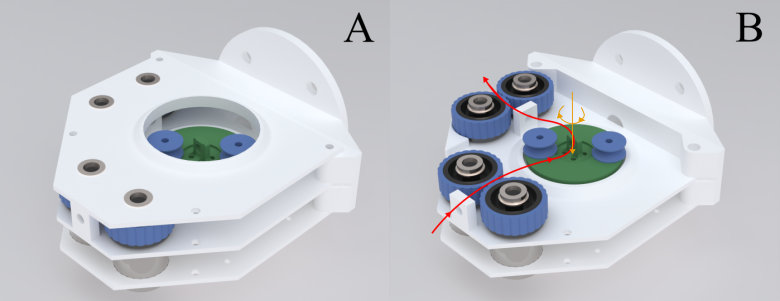
\includegraphics[width=\linewidth]{Figures/Figure11.png}
\caption{The friction wheels and the retraction mechanism driving motors are highlighted for illustration.}
\end{minipage}
\end{tabular}
\end{figure}

When retraction is required, the mechanism undergoes a coordinated sequence of actions. The rear pair of friction wheels maintains its rotational speed, continuing to pull the string inwards. Simultaneously, the front pair of wheels reverses direction, creating a counterforce that pulls the string loop into the space between the two pairs of wheels. This space is precisely designed to accommodate the retracted string without entanglement.

Within this confined space, a spool mechanism is designed. The spool is equipped with a rotational motor that winds the string onto itself, storing it neatly for future use. The tension exerted on the string during retraction is monitored by a force feedback sensor located on the spool's axle. This sensor is used to observe cable loading and support safety limits during the preprogrammed retraction sequence.

\subsection{Controller, Actuation, and Sensing Hardware}

The ESP32 main controller serves as the central hub for Lasso Gripper operations. It receives the experiment script or operator command, sends motor commands to the launch and retraction modules, and reads the sensing signals used for monitoring.
\begin{figure}[htbp]
\centering
\begin{tabular}{cc}
\begin{minipage}[t]{0.5\textwidth}
\centering
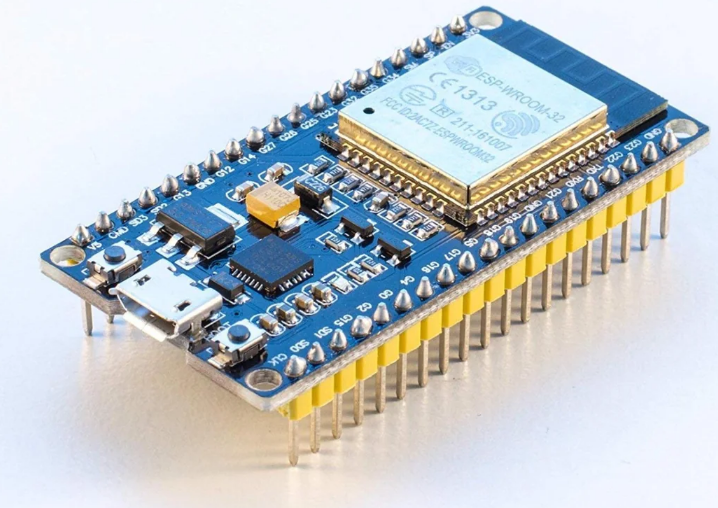
\includegraphics[width=\linewidth]{Figures/esp32.png}
\caption{ESP32 controller used in Lasso Gripper.}
\end{minipage}
\end{tabular}
\end{figure}
Its dual-core processor handles motor command execution, basic sensor monitoring, and communication with external devices. The controller interfaces with a spool-mounted force sensor, motor encoders, and any auxiliary trackers used during experiments.

GPIO pins drive the retraction modules and friction-wheel controllers, while PWM outputs provide fine speed control for the propulsion motors. Wireless connectivity is used for logging and remote monitoring via a host computer when required.

\section{Operational Workflow and Control Logic}
The operation of Lasso Gripper in the reported demonstrations was implemented as a preprogrammed launch, approach, retraction, lifting, and release sequence. The system did not autonomously recognize objects or decide when to grasp based on visual detection. Instead, the target position, approach direction, launch timing, retraction duration, and release command were specified before each trial according to the experimental setup. This section clarifies that control logic and distinguishes the implemented demonstration sequence from possible future closed-loop autonomy.

% ------------------------- 3.1 Demonstration Control Assumptions -------------------------
\subsection{Demonstration Control Assumptions}
The experiments were designed to validate the mechanical feasibility of loop-based capture rather than to demonstrate autonomous perception or decision making. Before each trial, the object was placed in a known region and the robot motion was manually selected or preprogrammed so that the open string loop would sweep across the intended capture region. For static targets, the launch and retraction timing were triggered by the experiment script. For moving-object demonstrations, the gripper was held at a fixed pose and the object was manually thrown through the loop during the launch window.

Sensors were used primarily for command execution, monitoring, and post-trial interpretation rather than for autonomous state transitions. Motor controllers provided speed and position control for the friction wheels and retraction spool. The spool-mounted force sensor was used to monitor cable tension and prevent excessive loading during retraction. Camera images and point-cloud examples were used to illustrate feasible loop placement and caging geometry, but the prototype did not use online object recognition to initiate grasping or release actions.

\subsection{Preprogrammed Grasping State Machine}
The demonstration controller can be described as a simple state machine with scripted transitions. The transitions are based on elapsed time, predefined motor commands, robot trajectory waypoints, operator commands, and safety limits rather than automatic visual recognition. The states are:
\begin{itemize}
    \item \textbf{Idle}: the controller waits for an operator start command.
    \item \textbf{Preset}: the target pose, robot sweep path, launch motor current, retraction motor current, and timing parameters are loaded into the experiment script.
    \item \textbf{Launch}: the friction wheels spin up and extrude the string to form the open loop.
    \item \textbf{Approach/Sweep}: for static objects, the robot follows the predefined path so that the loop passes around the target region; for moving objects, the gripper remains fixed while the object enters the loop.
    \item \textbf{Retract/Tighten}: the spool motor retracts the string according to the programmed duration or position command. Tension is monitored to avoid excessive load.
    \item \textbf{Lift/Transport}: after retraction, the robot performs the scripted lifting or transport motion.
    \item \textbf{Release}: the operator or script commands spool unwinding and friction-wheel reversal or relaxation, allowing the loop to reopen and release the object.
    \item \textbf{Recovery}: the string is rewound to the initial configuration and the controller returns to \textbf{Idle}.
\end{itemize}

The corresponding actuation and signal flow is summarized in Fig.~\ref{fig:grasp_release_flow}. The host script sends velocity or position commands to the ESP32 controller. The ESP32 drives the electronic speed controllers for the friction wheels and the spool motor driver for retraction. Sensor feedback is limited to motor state and cable tension monitoring; it does not trigger autonomous grasp initiation in the current prototype.

\begin{figure}[htbp]
\centering
\begin{tikzpicture}[
    node distance=0.5cm,
    every node/.style={font=\small},
    block/.style={draw, rectangle, rounded corners, align=center, minimum width=3.2cm, minimum height=0.85cm},
    arrow/.style={->, thick}
]
\node[block] (idle) {Idle\\operator start};
\node[block, below=of idle] (preset) {Preset trial\\pose, timing, speeds};
\node[block, below=of preset] (launch) {Launch loop\\friction wheels on};
\node[block, below=of launch] (sweep) {Approach / sweep\\predefined robot motion};
\node[block, below=of sweep] (retract) {Retract / tighten\\spool motor command};
\node[block, below=of retract] (lift) {Lift / transport\\scripted robot motion};
\node[block, below=of lift] (release) {Release\\unwind or relax string};
\node[block, below=of release] (recovery) {Recovery\\rewind and reset};

\draw[arrow] (idle) -- (preset);
\draw[arrow] (preset) -- (launch);
\draw[arrow] (launch) -- (sweep);
\draw[arrow] (sweep) -- (retract);
\draw[arrow] (retract) -- (lift);
\draw[arrow] (lift) -- (release);
\draw[arrow] (release) -- (recovery);
\draw[arrow] (recovery.east) -- ++(1.2,0) |- (idle.east);

\node[block, right=4.4cm of retract, minimum width=3.9cm] (monitor) {Monitoring only\\tension, motor state};
\draw[arrow] (retract.east) -- (monitor.west);
\draw[arrow] (monitor.south) |- (release.east);
\end{tikzpicture}
\caption{Preprogrammed grasping and release sequence used in the demonstrations. The current prototype does not autonomously detect objects or trigger grasping from visual feedback; state transitions are commanded by the operator or experiment script, with tension and motor signals used for monitoring and safety.}
\label{fig:grasp_release_flow}
\end{figure}

\begin{figure}[htbp]
\centering
\begin{tabular}{cc}
\begin{minipage}[t]{0.9\textwidth}
\centering
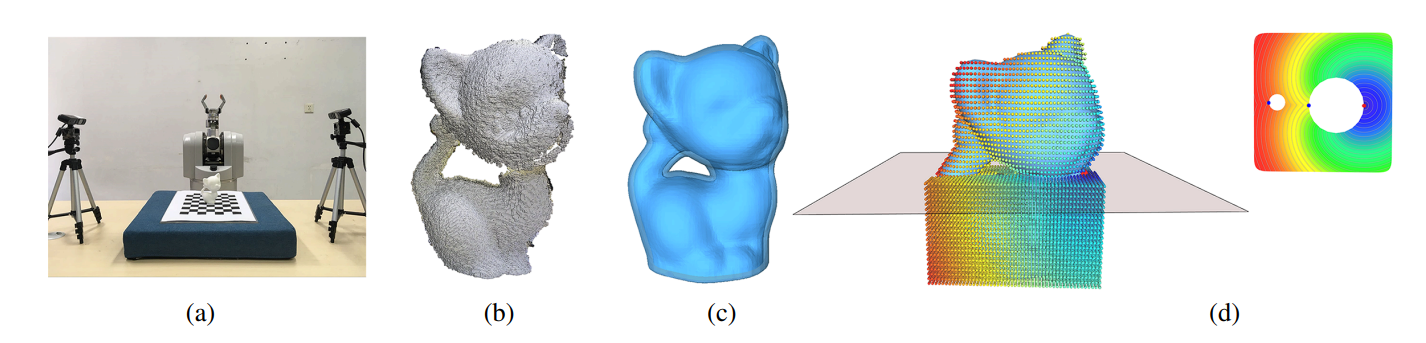
\includegraphics[width=\linewidth]{Figures/caging.png}
\caption{Caging-loop calculation algorithm for Lasso Gripper \cite{liu2018caging}. (a) Setup of the depth reconstruction system. (b) Point cloud captured directly by the depth camera. (c) An r-offset surface built to define the grasping space. (d) Two Morse saddle points (blue) calculated to define the grasping loop.}
\label{fig:caging_loop_method}
\end{minipage}
\end{tabular}
\end{figure}

The caging-loop concept shown in Fig.~\ref{fig:caging_loop_method} motivates the geometric placement of the loop around neck-like regions. In the present prototype, this concept was used to guide experimental setup and qualitative interpretation rather than as a fully automated online perception module. Future versions could integrate the point-cloud caging method with closed-loop planning, but this capability was outside the scope of the current demonstration.

% ------------------------- 3.2 Loop Positioning and Tightening -------------------------
\subsection{Loop Positioning and Tightening}

For the reported experiments, loop positioning was determined before each trial from the known target location and the intended capture region. The key requirement was to align the open loop so that retraction would cause the string to close around a neck, protrusion, or enclosed region of the object. This preplanned positioning was sufficient for demonstrating the mechanical advantages of distributed contact and large capture tolerance.

\begin{figure}[htbp]
\centering
\begin{tabular}{cc}
\begin{minipage}[t]{0.9\textwidth}
\centering
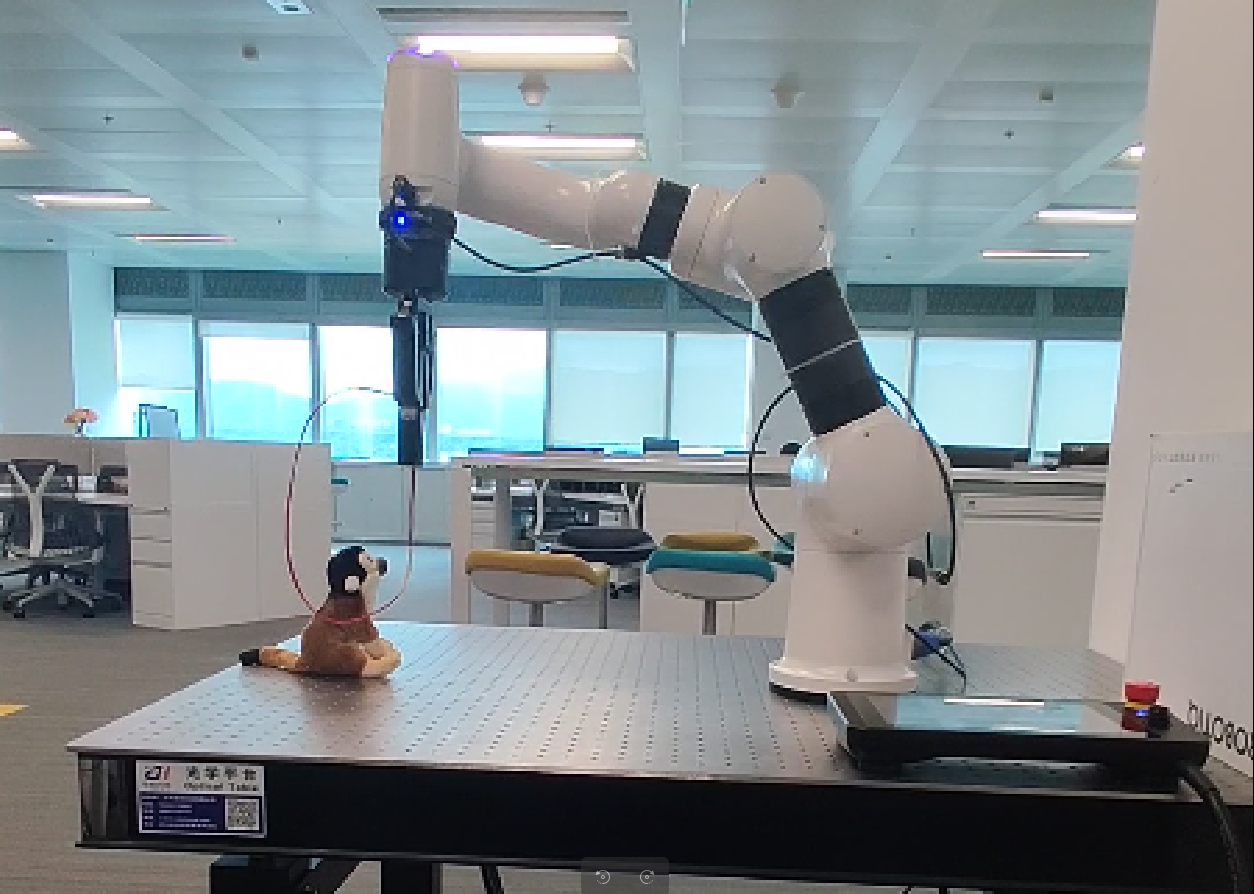
\includegraphics[width=\linewidth]{Figures/exp.png}
\caption{Illustration of the relative position of the string loop and the target object -- an early test}
\end{minipage}
\end{tabular}
\end{figure}

The tightening process is executed in a controlled manner, with the string loop gradually constricting around the target region. The wrist of the gripper approaches the object in synchrony with the programmed retraction action, ensuring that the loop maintains its position and grip.

% ------------------------- 3.3 Real-Time Feedback and Adjustment -------------------------
\subsection{Monitoring and Safety Feedback}
The current prototype uses feedback for monitoring and safety rather than autonomous grasp planning. The spool-mounted force sensor provides cable-tension information during retraction, while motor encoders provide actuator state information. These signals help verify whether the commanded sequence is being executed properly and whether the cable load remains within a reasonable range.

The force feedback sensor, located on the spool's axle, plays a safety role during tightening. If the measured tension exceeds a preset threshold, the controller can stop or relax the retraction command to reduce the risk of damaging the object or overloading the mechanism. In the reported demonstrations, this feedback was not used to automatically recognize successful capture; capture success was assessed from the observed outcome of the trial.

\section{Loop Dynamics and Workspace Extension}

The previous sections define the mechanical sequence used to deploy, position, and tighten the loop. This section explains why the deployed string can form a useful free-space shape and how that shape extends the effective workspace of a robot arm beyond the rigid wrist position.

\subsection{Dynamics of the String Loop}
This section analyzes the loop dynamics that govern Lasso Gripper operation. We focus on the transition from a gravity-dominated regime at low ejection speeds to a self-supporting regime at higher speeds, where aerodynamic drag and inertial effects stabilize the loop shape. The analytic model follows prior theoretical work and is compared with representative experimental profiles to validate qualitative trends \cite{abello2024string}\cite{daerr2019charmed}.

At low ejection speeds the loop sags under gravity. As ejection speed increases, aerodynamic drag and inertial forces can balance gravity and internal tension, yielding a self-supporting loop profile. Characterizing these regimes helps select launch speed, loop length, and control strategies that improve capture reliability.

\begin{figure}[htbp]
\centering
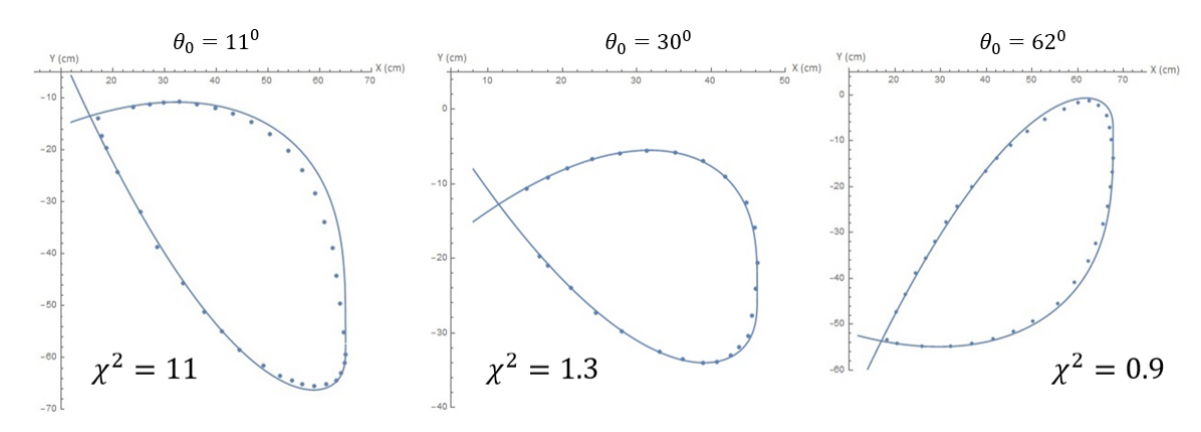
\includegraphics[width=\linewidth]{Figures/stringsim.png}
\caption{Comparison of numerical loop-shape solutions with representative experimental profiles \cite{abello2024string}. Example parameters: linear mass $\mu = 0.283 \pm 0.005\,\mathrm{g\,m^{-1}}$, loop length $L = 160\,\mathrm{cm}$, ejection speed $v = 5.1\,\mathrm{m\,s^{-1}}$, and several ejection pitch angles $\theta_0$. A satisfactory fit with $\chi^2 \leq 11$ was obtained for these samples.}
\label{simulation}
\end{figure}

Assuming the loop junction is at position $s = s_0$ when $t = 0$, the position of the junction along this curve is $s = v \cdot t + s_0 (\mathrm{mod} \, L)$. Denote $T(s)$ as the local tension. The Frenet--Serret frame $(\vec{\tau},\vec{n})$ describes an infinitesimal string element of length $\mathrm{d}s$ subjected to its weight $\mu\,\mathrm{d}s\,\vec{g}$, the local tension $\frac{\mathrm{d}(T\vec{\tau})}{\mathrm{d}s}\,\mathrm{d}s$, and a linear air drag $-f\,\vec{\tau}\,\mathrm{d}s$ with $f>0$.

Newton's motion equation produces:

\vspace{-0.3cm}
\begin{equation}
\begin{split}
\frac{\mathrm{d}(\mu v \vec{\tau})}{\mathrm{d}t} = \mu \vec{g} + \frac{\mathrm{d}(T \vec{\tau})}{\mathrm{d}s} - f \vec{\tau}
\end{split}
\end{equation}

Noting $\mathrm{d}s = v \cdot \mathrm{d}t$ and defining the effective tension $T^o = T-\mu v^2$, the following balance equation can be written:

\vspace{-0.3cm}
\begin{equation}
\begin{split}
T^o \vec{\tau} - f \vec{\tau} +\mu \vec{g}s=\vec{0}
\end{split}
\end{equation}

If the origin is wisely chosen for $\vec{r}$ as the point $o$ where the tangent to the loop is vertical, the integration constants will vanish. In the vertical local Frenet--Serret frame, defining $\tan\theta = \frac{\mathrm{d}z}{\mathrm{d}x}$, the following can be obtained:

\vspace{-0.3cm}
\begin{equation}
\begin{split}
-f \cdot ( x \tan \theta - z )+\mu gs=0
\end{split}
\end{equation}

This integro-differential equation admits analytical solutions under the stated simplifications; representative solutions are compared with experiment in Fig. \ref{simulation}.

The formation of the self-supporting loop is governed by aerodynamic drag acting on the string. Daerr et al. (2019) investigated this drag both experimentally and theoretically, focusing on a smooth long cylinder moving along its axis \cite{daerr2019charmed}. The drag arises from interaction between the moving string and the surrounding air, producing pressure and shear forces that can support the loop.

The loop-shape equations are formulated under the assumption of negligible string radius. They reveal a critical interface separating two regions: a supercritical zone (string speed larger than wave speed) and a subcritical zone (wave speed larger than local string speed). Regular solutions that cross this juncture continuously can be obtained and compared with experimental profiles.

In practical terms, understanding the string loop dynamics has significant implications for Lasso Gripper's design and operation. By leveraging the principles of aerodynamic drag and the transition between different velocity regimes, Lasso Gripper can achieve precise control over the string loop's shape and stability. This enables the gripper to handle objects with varying sizes and shapes effectively, improving robustness of capture.

\subsection{Workspace Analysis}
Because Lasso Gripper forms a self-supporting loop in three-dimensional space, the operational workspace of the proposed manipulator extends beyond the physical reach of the robotic arm.

\begin{figure}[ht]
    \centering
    
\includegraphics[width=0.8\linewidth]{workspace.png} 
    \caption{Lasso Gripper string loop is set at the end of UR5 robotic arm. The green point at the end of the robotic arm marks the position reachable by a rigid manipulator, while the red point indicates the furthest position on the string loop from the original point at the same robotic position.}
    \label{ws1}
\end{figure}

Consistent with the loop-dynamics analysis above, the three-dimensional pose kinematics of the lasso-type end-effector can be characterized by constrained dynamics under gravitational loading. For the local coordinate system constrained by gravity, the working plane is defined as the plane formed by the lasso's ejection direction and the gravity direction. The rotation with the normal vector of this working plane as the rotation axis is defined as pitch, while the rotation with the gravity vector as the rotation axis is defined as yaw. According to the right-hand coordinate system, the roll rotation axis is defined as the axis orthogonal to both the pitch and yaw rotation axes, lying within the working plane. Specifically, the gripper mechanism exhibits negligible roll angular displacement within the global coordinate frame due to gravitational stabilization. Its pitch orientation becomes parametrically dependent on the projectile's ejection velocity vector, while yaw angle variations are governed by the robotic manipulator's pose in Cartesian space.

\begin{figure}[htp]
    \centering
    
\includegraphics[width=0.6 \linewidth]{ws3.jpg} 
    \caption{The initial robotic arm workspace is marked in green, and the extended Lasso Gripper workspace is marked in red.}
    \label{ws2}
\end{figure}

A case study is conducted with specific parameters to investigate the workspace of Lasso Gripper on a 6-axis robotic arm using the Monte Carlo method. A UR5 robot without joint angle limits is used as an example in Fig. \ref{ws1}, and $[R, x_{+}, x_{-}]$ is set as $[0.7, 0.2\,m, 0.1\,m]$ in this case. The green point at the end of the robotic arm is the specific position that a rigid manipulator can reach, and the red point represents the furthest point on the string loop from the same robotic position. The sets of green and red points in Fig. \ref{ws2} are the workspace of the robotic arm and the extended workspace of Lasso Gripper, respectively. After generating 200,000 sampled robotic-arm configurations, the convex-hull workspace volume is calculated. The volume of the original UR5 workspace convex hull is $3.4620\,\mathrm{m^3}$, and the volume of the extended Lasso Gripper workspace convex hull is $8.9002\,\mathrm{m^3}$. The workspace extension ratio reaches $157.08\%$.
\section{Experimental Methodology}

The preceding sections establish the mechanism, control sequence, and loop behavior. The following experiments were designed to evaluate whether these elements can produce useful grasping outcomes under selected demonstration conditions.

\subsection{Experimental Objectives}
To validate the unique capabilities of Lasso Gripper and to compare its performance with antipodal grippers, the following experimental procedure was designed. The setup employed a modular robotic arm (Inovo Robotic) with a maximum payload of 6 kg, mounted on a flat platform where the target objects were placed.
The experimental objectives were divided into four categories:

    \begin{enumerate}
        \item Capturing animal figures by the neck or horns,

        \item Capturing objects of diverse shapes,

        \item Capturing oversized objects through shape adaptation, and

        \item Capturing moving objects.
    \end{enumerate}

\subsection{Experimental Setup}
For Objectives 1 to 3, the procedure consisted of the following steps:

    \begin{enumerate}
        \item The robotic arm moved to a predefined position to initiate the launch phase;

        \item Lasso Gripper was swept toward the target while maintaining its open-loop configuration;

        \item Upon reaching the target, the string was retracted to secure the object;

        \item The arm performed a vertical lifting motion while maintaining a stable grip.
    \end{enumerate}
For Objective 4, the robotic arm remained stationary, and Lasso Gripper independently executed the capture process aimed at intercepting a moving object in flight.
\paragraph{Control mode}
All demonstrations used a preprogrammed control sequence. The system did not autonomously detect the object or decide when to initiate grasping. Instead, the robot path, launch timing, retraction timing, and release timing were defined before each trial. The operator initiated the sequence, and the controller executed the scripted motor commands while monitoring cable tension and motor state for safety.
\subsection{Experimental Procedure}
The experimental procedure was divided into phases to evaluate Lasso Gripper's performance:
\begin{enumerate}
    \item \textbf{Static Object Gripping Tests}: Static object gripping tests were conducted to assess the gripper's ability to handle stationary objects. Test objects were placed in fixed positions, and the preprogrammed launch-and-retract sequence was executed to secure and lift each object. Success rates, gripping forces, and any slippage or deformation of the objects were recorded where feasible.

\item \textbf{Dynamic Object Gripping Tests}: Dynamic object gripping tests focused on evaluating the gripper's performance with moving objects. Test objects with controlled motion, such as rolling or sliding trajectories, were introduced and the lasso attempted to intercept and secure them. The effectiveness and speed of the gripping action were measured to assess performance in dynamic scenarios.

\item \textbf{Comparative Analysis}: Finally, a comparative analysis was conducted to compare Lasso Gripper's performance with traditional gripping methods. Parallel tests using a standard parallel-jaw gripper were carried out on the same set of test objects. Differences in gripping force, handling precision, success rates, and overall efficiency were analyzed to highlight advantages and potential areas for improvement of Lasso Gripper.
\end{enumerate}


\subsection{Data Collection and Analysis}
Data collection involved capturing both quantitative and qualitative metrics where available. Key observations included whether the loop enclosed the intended target region, whether retraction produced a stable hold, whether the object could be lifted or transported, and whether visible damage, deformation, slippage, or entanglement occurred. The spool force sensor provided cable-load information during retraction, while images and video frames were used to interpret loop placement around candidate neck, frame, or protrusion regions. Where feasible, counts of successful and failed grasps were noted; however, the evaluation emphasis in this section is demonstrative rather than a full statistical study.

Limited summary statistics were computed where appropriate, but a comprehensive statistical campaign (large-sample success rates, fatigue tests) was outside the present scope and is recommended for future work. Most representative scenes were repeated twice after the loop length and approach angle had been preset. This trial structure should therefore be interpreted as a repeatability check under selected demonstration conditions rather than as an unbiased statistical evaluation across random object poses.

\begin{table}[htbp]
    \centering
    \caption{Representative Lasso Gripper demonstration cases}
    \label{tab:lasso_demo_cases}
    \begin{tabular}{p{0.18\linewidth} p{0.12\linewidth} p{0.12\linewidth} p{0.16\linewidth} p{0.20\linewidth}}
        \toprule
        Target & Mass & Trials & Outcome & Notes \\
        \midrule
        3D-printed figures & 50\,g & 2 & 2 successful & Horn/neck capture \\
        DJI Mini 3 drone & 249\,g & 2 & 2 successful & Frame capture \\
        Cabbage & 170\,g & 2 & 2 successful & Irregular object \\
        Empty coke can & 305\,g & 2 & 2 successful & Cylindrical object \\
        Chili pepper & 90\,g & 2 & 1 secure, 1 slipped & Unbalanced mass \\
        Oversized balloons & -- & Example & Successful & Adaptive contact \\
        Thrown balloons & -- & Example & Successful & Moving target \\
        \bottomrule
    \end{tabular}
\end{table}

The table summarizes the representative cases used in this chapter. Because the approach angle and loop length were selected before each trial, the results should be interpreted as feasibility demonstrations under known setup conditions rather than as a randomized statistical evaluation. The detailed interpretation of these cases is presented after the experimental results.

\subsection{Experimental Parameter Selection}
Although the demonstrations were not designed as a large statistical campaign, several operating parameters were selected deliberately before each trial. These parameters determine whether the loop forms, reaches the target, tightens in time, and remains stable during lifting. The most important parameters are loop length, launch speed, approach angle, retraction timing, and lifting trajectory.

Loop length defines the size of the capture region. A longer loop increases the geometric tolerance to object-position error and makes it easier to capture oversized objects, but it also increases the risk of sagging, contact with the support surface, and entanglement during retraction. A shorter loop is easier to control and retract, but it requires more accurate placement around the target. For objects with clear neck or horn features, such as the 3D-printed bull and horse figures, a moderate loop length is sufficient because the loop only needs to pass around a narrow capture feature. For balloons or large irregular objects, a larger loop is beneficial because the target may not provide a precise narrow feature.

Launch speed affects whether the loop becomes self-supporting. If the speed is too low, gravity causes the loop to collapse before it sweeps across the target. If the speed is too high, the loop may become difficult to place accurately and may rebound after contact. The selected speed must therefore produce a loop that is large and stable enough for capture but not so aggressive that it destabilizes the approach. This trade-off is consistent with the loop-dynamics analysis presented earlier in the chapter.

Approach angle determines how the open loop intersects the object. For neck-like features, the preferred approach is one in which the loop plane crosses behind the feature and the retraction direction pulls the loop toward a mechanically stable region. For cylindrical or irregular objects, the approach angle must also consider the center of mass. The chili-pepper failure demonstrates this issue: even if the loop initially encloses part of the object, lifting can cause rotation if the tightened loop does not settle below or around a stable support region.

Retraction timing is the transition between geometric capture and force closure. Early retraction can close the loop before the target is fully inside the capture region, producing a miss. Late retraction can allow the target to leave the loop or allow the loop to slide to an undesired position. Retraction speed also matters. A slow retraction may fail to secure moving objects; a fast retraction may cause overshoot, local compression, or string shift. In the current prototype, these timing values were selected manually from preliminary trials and then held constant for the repeated demonstrations.

\begin{table}[htbp]
    \centering
    \caption{Role of main experimental parameters in demonstrations with Lasso Gripper}
    \label{tab:lasso_parameters}
    \begin{tabular}{p{0.20\linewidth} p{0.30\linewidth} p{0.32\linewidth}}
        \toprule
        Parameter & Increasing the parameter tends to & Practical risk if poorly selected \\
        \midrule
        Loop length & Increase capture area and pose tolerance & Sagging, surface contact, entanglement, slower recovery \\
        Launch speed & Improve loop support and reach & Overshoot, rebound, reduced placement accuracy \\
        Approach angle & Change intersection between loop and target feature & Missed capture or unstable tightening region \\
        Retraction delay & Allow target to enter the loop before closure & Late closure and target escape \\
        Retraction speed & Tighten faster and improve moving-object capture & Local compression, string slip, or object rotation \\
        Lifting path & Test whether capture remains stable under load & Slip if loop is not below a stable support region \\
        \bottomrule
    \end{tabular}
\end{table}

These parameters are coupled rather than independent. For example, a long loop may require a higher launch speed to remain self-supporting, but higher speed may require a gentler approach angle to avoid collision or rebound. Similarly, a late retraction may be acceptable for a stationary cabbage but unacceptable for a thrown balloon. For this reason, the current experiments should be interpreted as selected operating demonstrations. They identify feasible parameter combinations and observed failure boundaries, but they do not yet define a complete parameter map.

\subsection{Success Criteria and Failure Taxonomy}
To make the demonstration results interpretable, success was defined as completion of the intended capture-and-lift sequence without object escape or visible damage. A trial was considered successful when the loop enclosed the target region, retraction generated a stable hold, and the robot lifted or transported the object through the scripted motion. A trial was considered partially successful when the loop initially captured the target but the object slipped, rotated out, or could not be transported reliably. A trial was considered failed when the loop missed the target, tangled, or could not close around a mechanically useful region.

This definition is deliberately task-based rather than purely geometric. A loop that touches the object is not necessarily a successful grasp. The loop must also settle into a stable force path that supports the object during lifting. Conversely, the loop does not need to achieve classical antipodal force closure at two precise points. Its advantage is that it can use distributed contact and caging-like enclosure to tolerate uncertainty.

\begin{table}[htbp]
    \centering
    \caption{Failure taxonomy for loop-based capture}
    \label{tab:lasso_failure_taxonomy}
    \begin{tabular}{p{0.22\linewidth} p{0.32\linewidth} p{0.30\linewidth}}
        \toprule
        Failure type & Typical cause & Design or control implication \\
        \midrule
        Geometric miss & Loop does not intersect a valid capture region & Improve approach planning and loop placement \\
        Premature closure & Retraction begins before target enters the loop & Delay retraction or use visual/tension trigger \\
        Late closure & Target leaves the loop before tightening & Shorten delay or increase retraction speed \\
        Slip after capture & Loop settles above center of mass or on low-friction region & Select lower support region or add multi-loop capture \\
        Entanglement & Long loop contacts fixtures, table, or gripper body & Limit loop length and improve recovery path \\
        Excessive compression & Retraction tension is too high for soft targets & Add tension regulation and object-dependent limits \\
        Dynamic escape & Moving target crosses loop too quickly or off-axis & Increase capture window or add tracking feedback \\
        \bottomrule
    \end{tabular}
\end{table}

The taxonomy helps explain why a simple success count would be insufficient at this stage. Two failures may both appear as unsuccessful grasps, but they can require different design responses. A geometric miss suggests a planning or sensing problem. A slip after capture suggests a stability or center-of-mass problem. Excessive compression suggests a tension-control problem. Entanglement suggests a loop-length and recovery-path problem. Distinguishing these categories is necessary before the mechanism can be improved systematically.

\section{Experimental Results}
% (paragraph will be indented)
The evaluation reported in this section is demonstration-focused and intended to validate feasibility, illustrate common operating modes, and highlight comparative behavior versus conventional antipodal grasping. Test cases emphasized scenarios where a loop-based capture offers clear mechanical advantages. Results are presented as illustrative sequences and representative frames rather than as full statistical studies. Observed failure modes (entanglement, missed captures at extreme approach angles, and tension-management lapses) are documented to guide design improvements.
\subsection{Various Objects Grasping Results}
\begin{figure}[htbp]
    \centering
    
\includegraphics[width=0.7 \linewidth]{test3.png}
    \caption{Validation of grasping ability via bull and horse figures.}
    \label{fig:3}
\end{figure}

\begin{figure}[htbp]
    \centering
    
\includegraphics[width=0.7 \linewidth]{test1.png}
    \caption{Validation of grasping ability over variable shapes: drone, cabbage, coke can and chili pepper.}
    \label{fig:4}
\end{figure}

\begin{figure}[htbp]
    \centering
    
\includegraphics[width=0.7 \linewidth]{test2.png}
    \caption{Validation of grasping ability with oversized objects: inflated balloons.}
    \label{fig:5}
\end{figure}
Fig. \ref{fig:3} illustrates the experimental results for Objective 1. The lasso attached to the horns and necks and secured the figures, allowing the robot to lift and transport them from the platform. These approximately 50\,g figures were useful because the horn and neck features provided repeatable geometric regions for loop closure. For the second set of target objects (a drone, a cabbage, an empty coke can, and a chili pepper), Lasso Gripper was tested on objects with more varied geometry and mass. The drone weighed approximately 249\,g, the cabbage approximately 170\,g, the empty coke can approximately 305\,g, and the chili pepper approximately 90\,g. Under the preset loop length and approach angle, the drone, cabbage, and coke-can cases were each completed successfully in two repeated trials. The chili pepper was less stable: one trial slipped out of the loop after capture because its mass distribution was uneven and the loop tightened around a region that did not remain below the center of mass during lifting.
\begin{figure}[htbp]
    \centering
    
\includegraphics[width=0.7 \linewidth]{test4.png}
    \caption{Flying object is captured by Lasso Gripper.}
    \label{fig:6}
\end{figure}
The grasping strategy for these experiments was similar. In both cases, the robot swept above the target while Lasso Gripper maintained the string in its full range, ensuring that the target could be captured as the string retracted. This strategy was extended to expansive targets such as oversized balloons. The third set comprised two flower-shaped balloons (diameters 45 cm and 71 cm) and a spike ball of 18 cm diameter, as shown in Fig. \ref{fig:5}. Although Lasso Gripper could not fully encircle the largest balloons due to loop-size limitations, the loop still secured them sufficiently to lift them from the platform. This observation led to the fourth case, capturing flying objects. Fig. \ref{fig:6} shows examples where a long balloon and a small flower balloon were manually thrown through Lasso Gripper's loop and successfully intercepted.

Some notable phenomena were observed during the demonstrations, illustrating additional advantages of Lasso Gripper. The string's sustained high speed made it possible to grasp objects placed close to surfaces. In Fig. \ref{fig:4} (B) and (D), where the cabbage and chili pepper were placed near the table, Lasso Gripper maintained the loop shape and achieved successful grasps despite limited clearance between the object and support surface. The adaptive, distributed contact provided by the loop tolerated deviations in placement; compared with the grasp posture in Fig. \ref{fig:5} (D), the loop in Fig. \ref{fig:5} (C) exhibited an unexpected pose deviation yet still produced a secure grip. Thus, Lasso Gripper demonstrates adaptive force-closure behavior.

The failure modes observed in the demonstrations were also informative. First, the loop may miss the target if the preset approach path does not sweep across a valid caging region. Second, even when the loop initially catches the object, a strongly unbalanced target can rotate during lifting and shift the loop toward an open end, as observed in the chili-pepper case. Third, excessive retraction can produce unnecessary local compression on soft objects, while insufficient retraction may leave the loop too loose for transport. These limitations motivate future closed-loop planning and tension regulation, but they do not undermine the main mechanism result: a simple tensile loop can provide a large capture region and distributed contact without requiring precise antipodal point placement.

\subsection{Comparison with Antipodal Point Gripper}

\begin{figure}[htbp]
    \centering
    
\includegraphics[width=0.7 \linewidth]{compare.png}
    \caption{The inflated balloon is captured by the antipodal gripper. As a result of the concentrated stress applied, the balloon was severely deformed.}
    \label{fig:7}
\end{figure}
As the comparison group, the 2F-140 gripper from Robotiq was used as the classical antipodal gripper. In this scenario, the small flower balloon served as the target due to its elasticity. As shown in Fig. \ref{fig:7}, the flower balloon experienced severe deformation when grasped by the antipodal gripper. Although the balloon remained intact after the trial, the limitation of traditional grippers for delicate or highly deformable objects was evident. Instead of concentrating forces on small contact patches, Lasso Gripper captures objects via distributed rope tension, avoiding damage to delicate surfaces and enabling handling of larger, potentially heavier objects than some traditional grippers.

\section{Discussion and Mechanism-Level Implications}

\subsection{Interpretation of Demonstration Evidence}

The experimental evidence in this chapter should be read as mechanism validation. The goal is to show that a launched tensile loop can create capture behaviors that are difficult for conventional point-contact grippers. The results are not intended to prove deployment-level reliability. This distinction matters because Lasso Gripper has a large operating space: object shape, object mass, center-of-mass location, surface friction, target motion, loop length, launch speed, approach direction, retraction timing, and lifting trajectory can all affect the outcome.

The demonstrations nevertheless support several specific claims. First, loop-based capture can use object features that are not suitable for antipodal grasping. Horns, necks, drone frames, and irregular vegetable surfaces all provide candidate regions for loop closure. Second, distributed contact can reduce local deformation compared with point-contact grasping, as illustrated by the balloon comparison. Third, the gripper can interact with targets that exceed the convenient opening range of a parallel-jaw gripper because the functional capture region is defined by the deployed loop rather than by rigid jaw spacing. Fourth, the same mechanism can capture both stationary and moving objects when the timing is preset appropriately.

\begin{table}[htbp]
    \centering
    \caption{Evidence interpretation for representative target categories}
    \label{tab:lasso_evidence_interpretation}
    \begin{tabular}{p{0.22\linewidth} p{0.30\linewidth} p{0.30\linewidth}}
        \toprule
        Target category & Mechanism behavior demonstrated & Remaining validation gap \\
        \midrule
        Horned and necked figures & Capture using protrusions and enclosed regions & Randomized pose and feature-size tolerance \\
        Drone frame & Capture of sparse frame-like geometry & Robustness to propeller guards, cables, or fragile components \\
        Cabbage and coke can & Handling of irregular or cylindrical objects & Surface-friction and mass-distribution sensitivity \\
        Chili pepper & Identification of slip due to asymmetric mass distribution & Stable capture planning around center of mass \\
        Oversized balloons & Distributed contact over targets larger than rigid gripper opening & Tension limits for fragile deformable objects \\
        Thrown balloons & Moving-target interception under preset timing & Closed-loop tracking and automatic trigger timing \\
        \bottomrule
    \end{tabular}
\end{table}

The results therefore justify the mechanism concept and motivate a more quantitative next phase. Future experiments should randomize object pose and approach direction, repeat each condition over larger trial counts, and record loop state, cable tension, object motion, and failure category. A meaningful quantitative campaign would report not only success rate but also the parameter boundary at which the loop transitions from reliable capture to miss, slip, or entanglement.

\subsection{Comparison Criteria for Loop and Antipodal Grippers}

The comparison between Lasso Gripper and the Robotiq 2F-140 gripper is qualitative, but it can still be framed using explicit criteria. A parallel-jaw gripper is strong and repeatable when it can place its fingertips at suitable contact points. Its main limitation appears when the object is too large, too deformable, moving, or difficult to access from two opposing sides. Lasso Gripper has the opposite profile. It does not provide the same precise fingertip placement, but it can define a larger capture region and distribute contact through a flexible loop.

This difference means that the two grippers should not be evaluated only by peak grip force. For deformable or fragile targets, a high local grip force can be undesirable. For oversized targets, jaw opening may be more limiting than motor force. For moving targets, capture-region size and timing may matter more than fingertip accuracy. For frame-like objects, the ability to pass through or around an opening can be more important than surface friction.

\begin{table}[htbp]
    \centering
    \caption{Qualitative comparison criteria for Lasso Gripper and antipodal grippers}
    \label{tab:lasso_antipodal_criteria}
    \begin{tabular}{p{0.24\linewidth} p{0.29\linewidth} p{0.29\linewidth}}
        \toprule
        Criterion & Lasso Gripper tendency & Antipodal gripper tendency \\
        \midrule
        Capture region & Large, loop-defined, tolerant to moderate pose error & Limited by jaw opening and fingertip placement \\
        Contact distribution & Distributed along string-object contact path & Concentrated at two main contact patches \\
        Deformable-object handling & Can reduce local deformation if tension is limited & Can deform object under high local pressure \\
        Oversized-object handling & Possible if loop can partially enclose or hook feature & Limited by maximum jaw opening \\
        Moving-object capture & Possible with large loop and correct timing & Requires accurate tracking and fingertip placement \\
        Precision placement & Lower, because loop shape is flexible & Higher when object geometry is known \\
        Failure mode & Miss, slip, entanglement, excessive loop tension & Missed fingertips, crushing, slipping from point contacts \\
        \bottomrule
    \end{tabular}
\end{table}

This comparison clarifies the intended contribution. Lasso Gripper is not proposed as a universal replacement for antipodal grippers. It is a complementary end-effector for tasks where capture tolerance, distributed contact, and geometric enclosure are more valuable than precise fingertip placement.

\subsection{Mechanism Contribution of Lasso Gripper}

Work on Lasso Gripper provides the main mechanism contribution of this thesis and offers several insights that generalize beyond the specific prototype. First, the principle of using a flexible tensile element to create an adaptive capture region suggests new ways to trade capture range for control complexity. Second, proximal actuation enables low distal mass while still producing useful end-effector behavior through a flexible transmission path. Third, performance metrics such as capture probability, peak tensile load, retraction dynamics, and hysteresis in the string path form a compact evaluation set that is applicable to other tendon-driven designs.

Taken together, these demonstrations support the feasibility of Lasso Gripper as a novel end-effector centered on adaptive loop capture. The results show that controlled tension, distributed contact, and low-distal-complexity actuation can produce robust behavior under uncertainty in object size, shape, and motion. The following chapter should therefore be read as a complementary application case within the same tendon-driven mechanism framework, not as a device derived directly from Lasso Gripper. The two systems occupy different roles in the thesis: Lasso Gripper is the primary exploratory and innovative platform, while the handheld surgical instrument is a secondary, application-oriented engineering implementation that examines guided cable transmission, packaging, and control under medical-device constraints.
